\chapter{相关技术和方法}
本文已在绪论\ref{subsec:面诊系统}中介绍了当前面诊系统现状,本章则关注于介绍本文用到的相关技术和方法。
在本文研究内容中,首次将技术探针的方法用于研究日常场景中的面诊系统设计问题,因此第一部分介绍技术探针相关知识及数据获取方法;
其次本文提出了通用可拓展的面诊系统设计并进行了实现,因此第二部分将介绍面诊系统相关技术;最后部分介绍系统设计中用到的方法和概念。

\section{技术探针}
% 为什么要用技术探针
日常场景下的面诊系统设计,涉及到用户行为模式分析,日常场景存在环境复杂,难以获取用户真实想法等挑战。

技术探针有一套激发用户参与设计、获取复杂日常场景下用户数据的方法论,本小节将简单介绍本文使用的技术探针及数据获取方法。

\subsection{技术探针简介}

通常,典型的人机交互领域中研究系统设计是访问用户的家庭,然后设计并实现一个系统让用户评价。
在日常场景下,这种设计方法缺点非常明显\cite{Hutchinson2003Technology}:
(1)没有激发用户的思考,可能无法反映用户的实际需求和掩盖在家庭内部之间更加有趣的设计。
(2)在设计和实现系统过程中,没有提供真实的长期使用场景,用户缺乏参与性。

\begin{figure}[h]
    \centering
    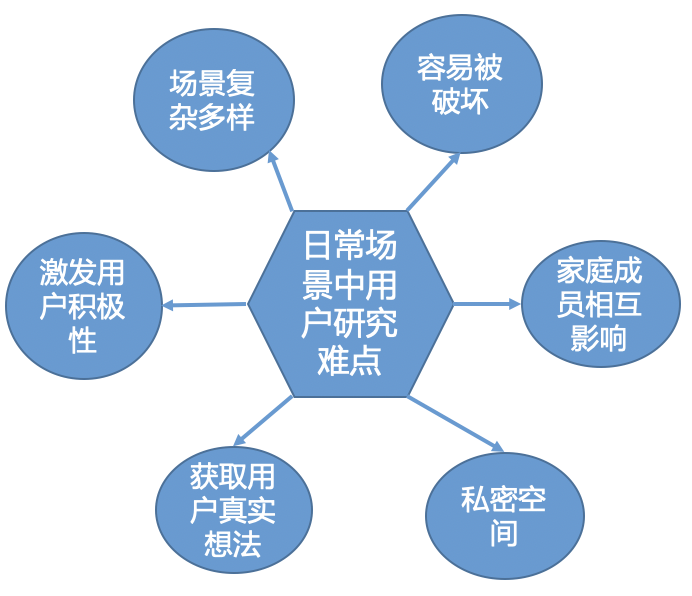
\includegraphics[width=6cm]{images/user_study_hard.png}
    \caption{日常场景中用户研究的难点}
    \label{fig:user_study_hard}
\end{figure}

如图\ref{fig:user_study_hard}所示,在日常场景中,用户的个人爱好、性格,家庭环境都不尽相同,家庭成员之间也互相联系。特别是考虑到日常长期使用场景,传统的研究方法容易破坏真实环境,并不能激发用户内心真正的需求和积极参与性。
在复杂的日常和私人环境下,了解用户对于面诊交互技术的需求和态度更加具有挑战性。此外,在研究某类技术新的场景时,如果该技术没有被广泛使用,直接对用户进行访谈无法获取相关数据。

% 介绍什么是技术探针
为了避免上述的问题,Hutchinson等\cite{Hutchinson2003Technology}提出了一种名为技术探针的研究方法:利用快速开发出来的、功能并不完善的简单系统,让用户在实际使用探针的过程中,鼓励用户大声表达自己真实的想法,在草稿上画出自己心中的系统,参与设计过程。
在人机交互中,技术探针是一种探索未知事物的工具。基于技术探针的方法主要用于系统设计的早期阶段\cite{turmo2020training},也经常被用来为日常使用的健康技术的设计提供信息。
目前已有不少成功使用案例,例如通过技术探针的设计方法,Papi等\cite{papi2015knee}利用可穿戴式膝关节技术探针,探索了在家庭环境下如何设计用于骨关节炎患者的康复工具;同样,Singh等\cite{singh2017supporting}通过1-2周的用户研究,利用技术探针,研究了如何设计慢性疼痛患者使用的日常可穿戴设备。

% 技术探针与原型的不同点
\subsection{技术探针特点与要求}
% 目前已有工作的不足之处

原型系统是在软件工程中,为了方便所有参与项目的成员如客户、开发者对系统功能达成共识,从而构建的最小化的系统模型。
而技术探针通过一个功能简单的系统,让用户在真实的场景中使用,鼓励用户大声说出自己的想法,并在纸上纪录下来,从而收集用户真实反馈,同时引导用户参与设计的过程。

为了帮助更好地理解技术探针,此处通过对比一下人机交互领域中的技术探针和计算机领域中的原型系统,以此说明为何以往的基于原型系统的面诊系统研究会在系统设计层面存在不足之处,同时体现技术探针的特点和要求。
与原型系统相比,技术探针的不同之处及要求在于:
\begin{enumerate}
    \item 系统定位。原型系统的目的是实现系统的几个基本功能,给用户介绍系统目前的能力,让用户体验系统。技术探针的定位是一个采集信息的工具,用来帮助确定未来的设计方案。因此对于技术探针来说,研究者可能一开始并不知道该系统应该如何设计,所以在实现一个技术探针时,功能应该尽可能简单,减少模块分层,把设计过程让用户自由发挥,不限制用户的使用方式。

    \item 功能可用性。对于原型系统来说,系统中的几个功能需要保证正常可用,才能算是一个合格的原型系统。但是对于技术探针说来,技术探针在设计的时候,是允许特意出现非常反人类的设计或者功能不符合预期的情况,以提前激发用户发表自己的设计意见。

    \item 与设计方案的关系。原型系统和技术探针,与设计方案的关系不同。技术探针出现在设计阶段之前,用于获取信息指导如何设计。原型系统在设计阶段之后,原型系统根据设计方案进行实现。
\end{enumerate}

此外,技术探针通常需要记录用户的操作日志,用于分析用户的行为,帮助产生新的设计;原型系统虽然也会记录日志,但用户操作日志通常用于记录信息与排查错误。

\subsection{数据获取与分析方法}
在计算机领域,常见的用户数据获取是通过大量统计数据,如大批量结构化的问卷、用户行为日志等,然后在分析过程中,通过提取自变量、因变量做变量的相关性分析得到最终的结论。
在人机交互中,通常采用获取数据的方法是通过资料分析、案例分析、直接观察、用户访谈等方式获取研究数据。
其中,深度访谈是人机交互领域中收集数据最常用的一种方式,通过开放式、半结构化的面对面访谈,能够深度了解调查者内心的客观想法,避免研究者的主观判断。
该方法在心理学与社会学领域被广泛应用,能够发掘出用户更细节的需求和想法。
同时,在挑选了足够的代表性采访对象的前提下,该方法相对地对数据量的要求不高,在连续访谈得到的结果相对稳定后可停止访谈\cite{cleary2014data}。
本文使用两者相结合的方式:在使用技术探针进行实验之后,首先通过分析日志和问卷,得到大致的结论,然后通过面对面深度访谈发掘更深层次的原因,得到最终的结论。

\section{云中医诊断模型}
本文采用技术探针的方法研究面诊技术在日常场景应用问题,因此在模型选取方面更加关注其面诊流程覆盖度以充分获取用户的数据。
云中医是复旦大学与上海中医药大学为社区与诊所环境共同研发的面诊系统,云中医的诊断模型不依赖特定的设备,实现了基本的体质诊断功能,准确率已经满足技术探针可以使用的需求,
且属于校内自己开发的平台,因此本文最终选择在云中医的基础上进行用户研究。

\begin{figure}[htb]
    \centering
    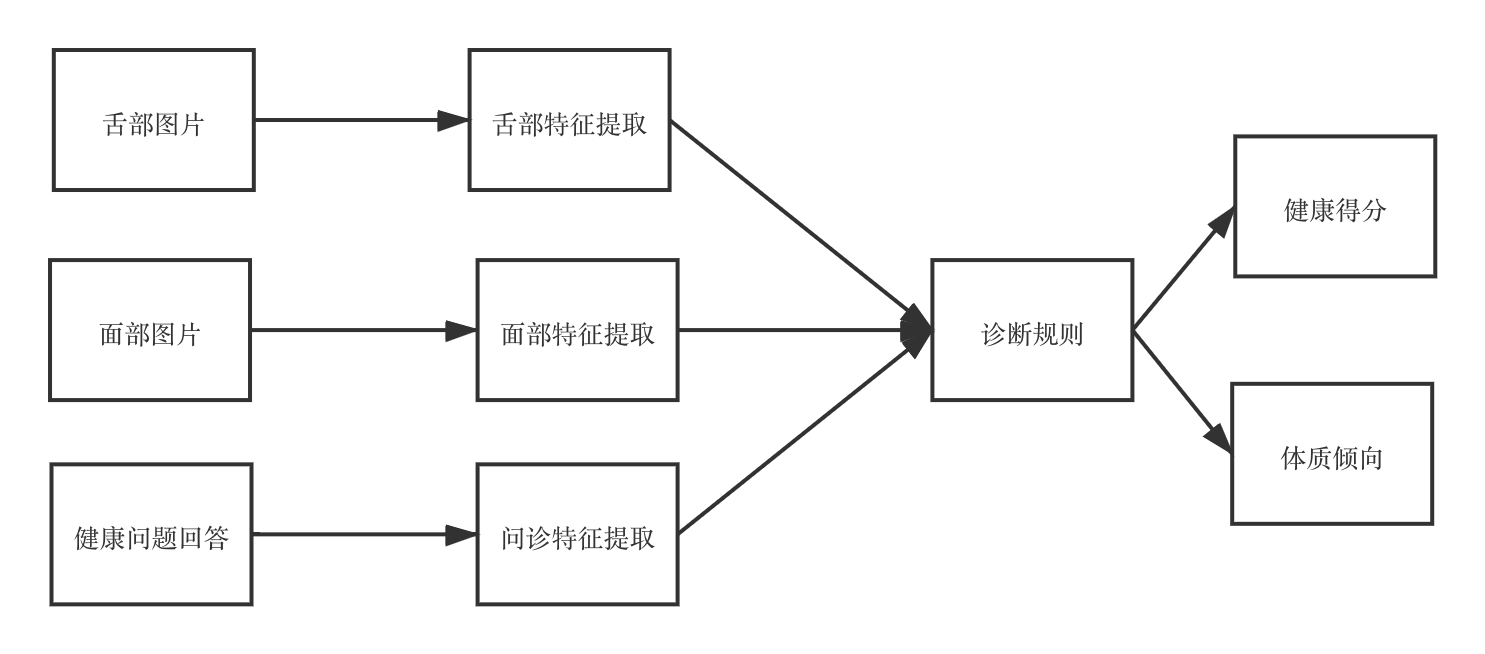
\includegraphics[width=15cm]{images/cloud_med3.png}
    \caption{模型处理流程}
    \label{fig:cloudmed1}
\end{figure}

如图\ref{fig:cloudmed1}所示,技术探针所用模型以面部图片、舌部图片、问诊问题作为输入,通过特征提取后由诊断模型与规则系统得到最终的体质和健康得分。
本文主要工作之一是研究面诊技术在日常场景下如何应用,利用云中医作为技术探针发现了目前面诊技术存在的各方面的问题并提出设计策略。
云中医中诊断模型详细内容由于篇幅较长,同时为明确与本文工作的关系,统一放在附录\ref{ch:appendix}中介绍。

下面简单介绍部分技术探针所用到的相关技术。
\subsection{特征提取}
颜色模型是用数值描述颜色的数学模型,当前主要使用的颜色模型有LAB, RGB、HSV、YCbCr等,
如HSV颜色模型中颜色由色相(H)、饱和度(S)、强度值(V)三个维度组成\cite{dhivakar2015face};而LAB颜色空间中L表示亮度通道,A与B分别代表红绿与蓝黄颜色通道。
LAB颜色空间是一种基于生理特征的颜色空间,常被用于人的肤色特征提取。

Haar级联检测器通常用于提取边缘特征比较明显,具有固定图像特征的兴趣区域,如从背景图中检测出人脸、舌部矩形区域等\cite{2001Rapid, 2007Learning}。
Haar特征可用于描述图像中的边缘、中心以及线性特征,通过级联分类器对图像的Haar特征值窗口扫描完成对应的目标检测。

此外,基于混合高斯模型的方法\cite{Hu2016Robust}也常用于不规则区域的提取。
混合高斯模型将图像抽象为多个高斯模型的线性叠加,可用于建立肤色区域建模。
在完成兴趣区域建模后,通过计算图像中每个像素点数据属于模型分布的概率,可将兴趣区域从背景中提取出来。

\subsection{诊断模型}

早期的面诊系统一般通过诊断规则实现。诊断规则即通过专业的医学知识编写的一系列规则,是通过分析大量的临床医疗数据以及现有的结论,将诊断特征与诊断结果的关系进行量化\cite{牛欣2011中医四诊合参辅助诊断关键技术的数字化、量化研究}。
由人工编写的一些固定规则,结合了人工的经验,能提供基本的诊断能力,但由于严重依赖规则、表达能力有限,目前主要用于减少其他模型的训练成本以及修正最终的结果。
目前各类诊所环境中使用的面诊仪,其主要用到的技术是通过上述的人脸检测、预处理和简单分类模型抽取特定特征,如面色、舌苔形状等,
然后系统通过一定规则提示医护人员相关信息,帮助医护人员判断健康情况。
如基于上文提到的颜色模型结合简单的规则,就能完成对慢性肾炎\cite{周小芳2019慢性肾功能衰竭患者虚兼湿浊证的面部色诊研究}、
冠心病\cite{陈聪2019冠心病痰瘀互结证面诊图像特征参数分析}等基本判断。

SVM\cite{cortes1995support}是统计学习方法中常用的分类模型,应用非常广泛。
SVM利用核函数将原始数据映射到高维空间,通过EM(Expectation-Maximum)算法求解一个超平面,完成对原始数据的分类,能够在小样本、非线性的情况下保持优秀的泛化能力。
将面诊问题抽象为分类问题,可使用分类模型抽取相关特征以及判断用户的体质类型、五脏特征等。
如陈淑华等\cite{chen2016facial}使用了SVM分类器\cite{cortes1995support}用于判断用户是否患有糖尿病、乳腺癌、胃炎等五种疾病,
在其数据集上判断健康与非健康能达到70\%的准确率,五种疾病平均准确率能达到79\%左右。

技术探针所用诊断模型由SVM分类器与诊断规则组成,但在系统设计上需要兼容其他诊断模型,下面做简单补充介绍。
近年来,诊断模型发展迅速,出现了大量基于深度学习的诊断模型,如Liang\cite{liang2020oralcam}在移动设备上实现了OralCam系统:
该系统使用深度卷积神经网络判断用户口腔图片是否有口腔疾病的五个特征,从而帮助用户提高口腔健康意识。
端到端(即直接将面部图片进行输入,不做手动特征提取)的模型设计往往需要大量的样本数据支持,而迁移学习能降低模型对数据量的要求。
Jin\cite{jin2020deep}等根据地中海贫血、甲亢病人脸部数据集,将在人脸识别数据集上预训练的卷积分类模型,迁移到面诊场景用于通过面部图片判断地中海贫血、甲亢病等,
其准确率达到90\%, 优于专业医生进行面诊得到的结果。

面对上述功能各异、更新迅速的诊断模型,本文希望提供一种通用可拓展的面诊系统设计,
在系统设计层面解决日常场景下的交互问题(如提供基于系统设计的可解释性而不依赖具体模型),但又同时能提供对各种诊断模型的兼容与接入,
从而达到诊断模型更新变化并不影响系统设计的目的。因此下一小节将介绍本文在实现一个通用可拓展的面诊系统中用到的技术。

%\subsection{特征提取方法}

% 人脸检测是面诊技术中预处理的基本技术之一,用于在图像中标定人脸的位置和大小。
% 人脸检测可能会遇到人脸过多、奇怪表情、面部朝向姿态、光照、分辨率、肤色等问题,特别是在非标准环境下,从复杂的图象中精确定位到人脸是非常有挑战的事情。
% 总的来说,人脸检测可以分为基于特征和基于图像两类。
%面诊技术中特征提取主要用在人脸检测和兴趣区域提取两个步骤中。
%
%人脸检测可以分为基于特征和基于图像两类。(1)基于特征的方法通过提取图像的特征,然后将特征与人脸特征信息进行匹配,这类方法主要代表有基于颜色模型的人脸检测\cite{dhivakar2015face}、ASM(Active Shape Model)\&PDM(Point Distribution Model)\cite{kumar2019face}、基于Gabor滤波器的人脸检测\cite{sharif2011face}等。
%如基于颜色模型的人脸检测通过将人脸图像映射到三位颜色空间进行简单判断。人的肤色是人脸中的一个非常重要的特征,使用人脸的肤色作为特征处理虽然准确率不高,但是速度快,计算简单。
%当前主要使用的颜色模型有LAB、RGB、HSV、YCbCr等,以HSV颜色模型为例,HSV颜色模型中颜色由色相(H)、饱和度(S)、强度值(V)三个维度组成\cite{dhivakar2015face}。
%通过HSV颜色模型,可使用简单的规则过滤出肤色需要满足的条件。本文使用的特征提取方法在提取面色特征与唇色特征时使用了HSV与LAB颜色模型。
%(2)基于图像的方法人脸检测方法直接将输入图像与训练人脸图像进行匹配,这类方法主要代表有特征脸方法(EigenFace)\cite{mulyono2019performance}、Haar分类器\cite{priadana2019face}、基于人工神经网络\cite{farfade2015multi}的方法等。
%这类方法不事先定义人脸的特征,而是采用训练数据的方式从数据中学习人脸的特征分布,在提供足够训练数据的情况下准确率相对基于特征的方法有了很大的提高。
%云中医所用模型采用了Haar分类器的方法用于人脸检测与舌部区域检测。

% \begin{figure}[h]
%     \centering
%     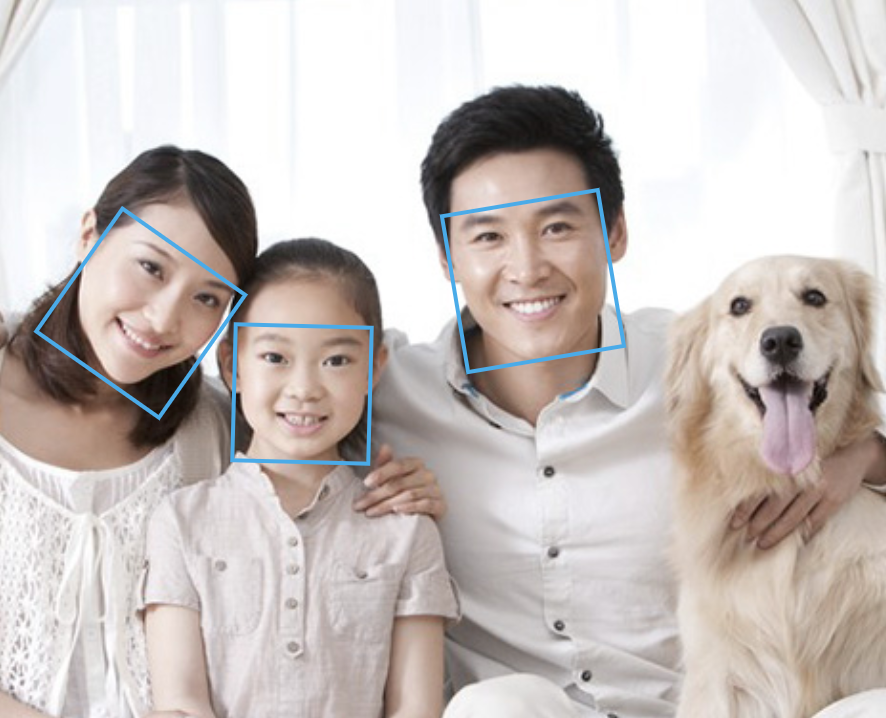
\includegraphics[width=8cm]{images/face_detcetion.png}
%     \caption{人脸检测 \protect\footnotemark}
%     \label{fig:face_plus }
% \end{figure}
% \footnotetext{https://www.faceplusplus.com.cn/}



% % \subsubsection{基于特征的人脸检测方法}
% 基于特征的方法通过提取图像的特征,然后将特征与人脸特征信息进行匹配,这类方法主要代表有基于颜色模型的人脸检测\cite{dhivakar2015face}、ASM(Active Shape Model)\&PDM(Point Distribution Model)\cite{kumar2019face}、基于Gabor滤波器的人脸检测\cite{sharif2011face}等。

% 基于颜色模型的人脸检测通过将人脸图像映射到三位颜色空间进行简单判断。人的肤色是人脸中的一个非常重要的特征,使用人脸的肤色作为特征处理虽然准确率不高,但是速度快,计算简单。
% 当前主要使用的颜色模型有RGB、HSV、YCbCr等,以HSV颜色模型为例,HSV颜色模型中颜色由色相(H)、饱和度(S)、强度值(V)三个维度组成\cite{dhivakar2015face}。
% 通过HSV颜色模型,使用简单的规则就可以过滤出肤色需要满足的条件:
% $$
% \left\{
% \begin{array}{c}
%     0 <= H <= 0.25 \\
%     0.15 <= S <= 0.9
% \end{array}
% \right.
% $$

% 基于Gabor滤波器的人脸检测则通过将人脸图像映射到特征图像进行对比。在图像处理中,Gabor滤波器常用于作为算子获取图像的边缘和纹理特征\cite{sahib2020hybrid}。
% 由于人脸有着独特的轮廓特征,因此Sharif等\cite{sharif2011face}提出了一个使用Gabor滤波器进行人脸检测的方法,
% 该方法使用40个Gabor滤波器为每个输入提供了40个特征图片,然后根据每个特征图片中强度最大的点与人脸库中对应的点进行距离比较,从而判断是否检测到人脸。

% 由上面两个例子可以看出,基于特征的人脸检测方法思想是尝试将人脸映射到另一个特征维度的以获取人脸的不变特征如眼睛、眉毛、嘴巴等,对特征脸的数据要求也比较小,实现起来简单。
% 但当人脸图像受到光线影响、被部分遮挡时,基于特征的方法准确率将大幅度下降。

% \subsubsection{基于图像的方法人脸检测方法}
% 基于图像的方法人脸检测方法直接将输入图像与训练人脸图像进行匹配,这类方法主要代表有特征脸方法(EigenFace)\cite{mulyono2019performance}、Haar分类器\cite{priadana2019face}、基于人工神经网络\cite{farfade2015multi}的方法等。
% 这类方法不事先定义人脸的特征,而是采用训练数据的方式从数据中学习人脸的特征分布,在提供足够训练数据的情况下准确率相对基于特征的方法有了很大的提高。

% Labeled Faces in the Wild (LFW)是著名的人脸识别测试集,一共有6000组人脸图像,其中包含一半的正样本和一半的负样本。
% 其中传统基于特征的检测方法,在LFW数据集准确率大概是60\%, 基于深度学习的检测方法普遍可以达到99\%以上的准确率,超过了人眼判断的97\%的准确率\cite{sun2015deeply}。


% \subsection{面部兴趣区域提取}
%兴趣区域提取在面诊技术中主要指的是从人脸图像中切分并提取出面部(去除五官)、舌部、唇部等不规则形状区域的技术,
%常见的方法有基于混合高斯模型(Gaussian Mixed Model)\cite{Hu2016Robust}、SegNet\cite{Badrinarayanan2017SegNet}、TCMINet\cite{li2020tcminet}等。
%本文中选用的模型,使用了基于混合高斯模型的兴趣区域提取方法提取唇部区域\cite{Hu2016Robust},该方法将人脸识别后的人脸图像拆分为上下两个部分,在上半部分利用混合高斯模型构建肤色分布,利用肤色分布在下半部分抽取唇部和舌部。
%基于混合高斯模型相比其它方法在准确率相对高的前提下鲁班性强且实现简单。
% \begin{figure}[h]
%     \centering
%     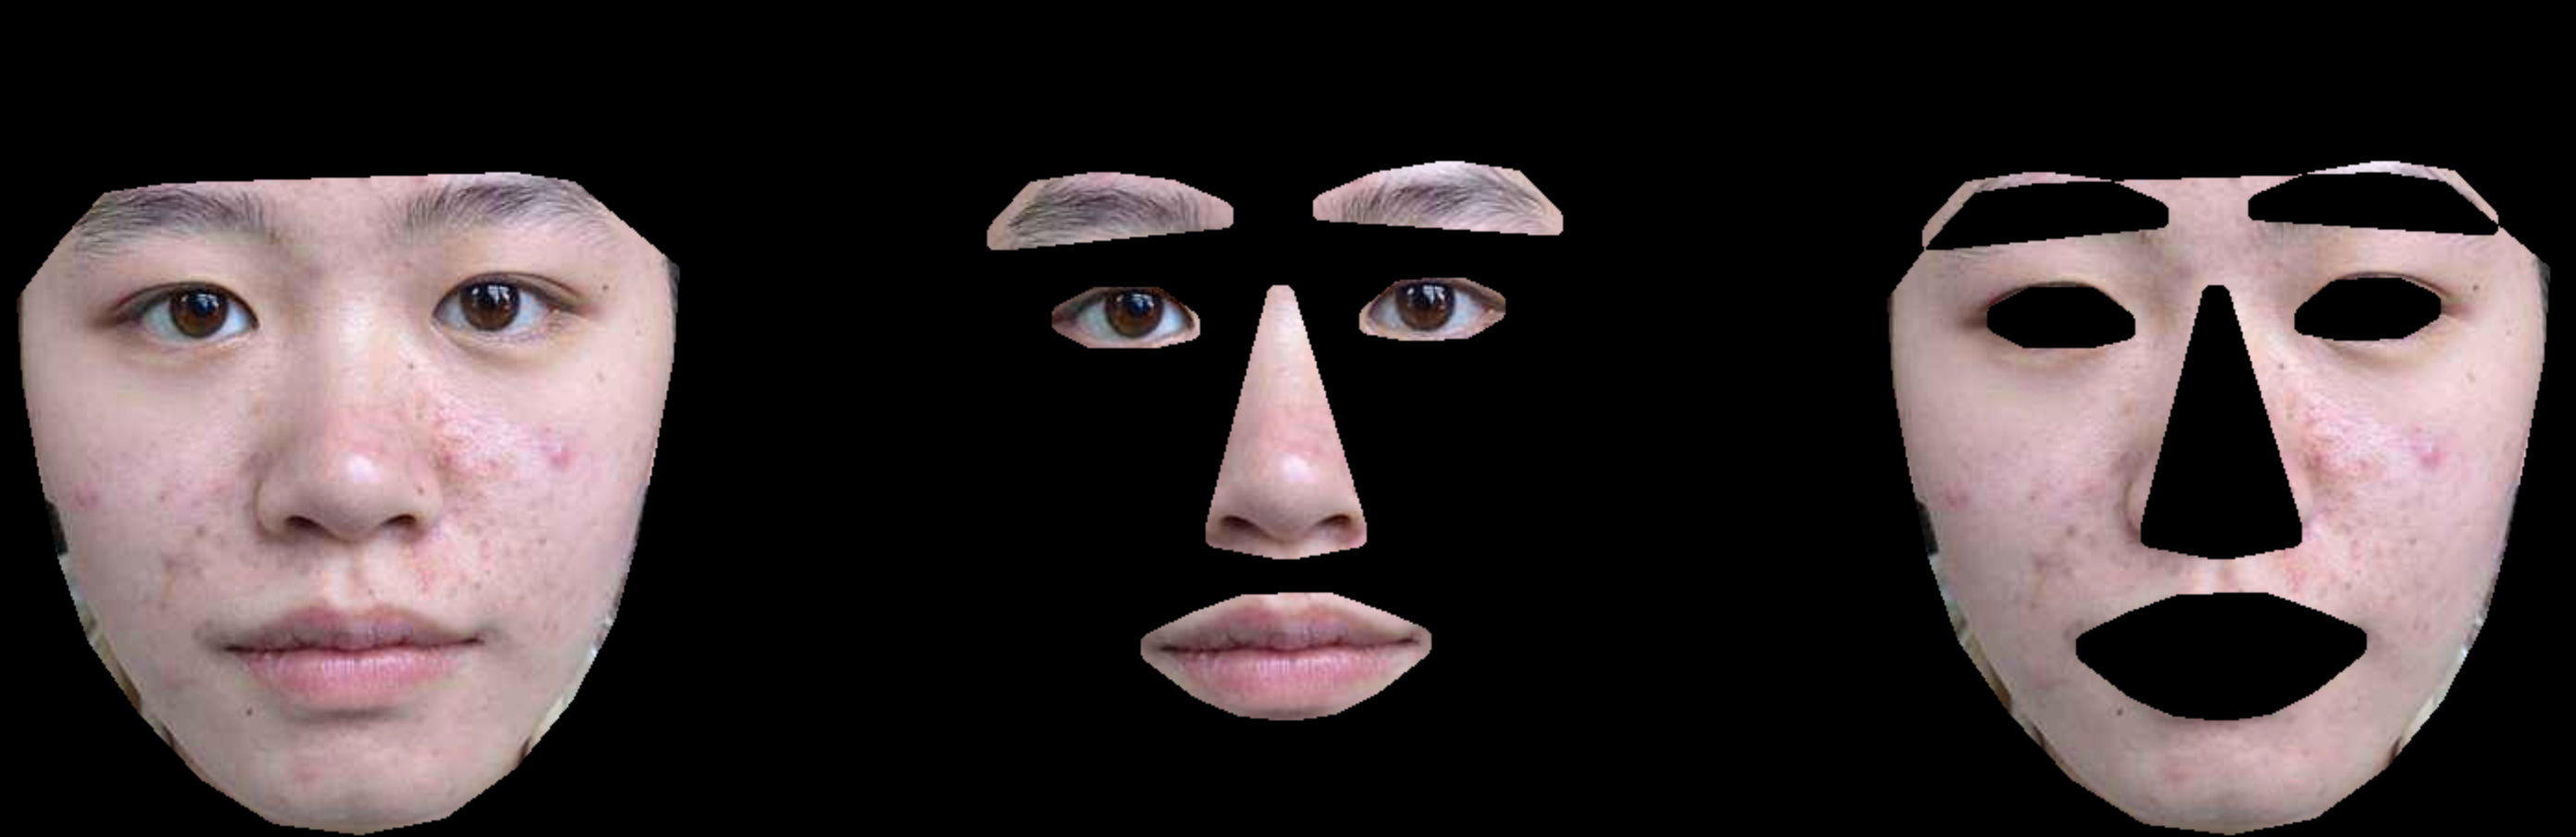
\includegraphics[width=12cm]{images/roi.png}
%     \caption{兴趣区域提取}
%     \label{fig:roi}
% \end{figure}

% 介绍单高斯模型


% 与面部图像预处理不同,特征提取算法主要关于点在于如何从图像数据中获取量化的基础特征,如面色、唇色、舌苔类型等。

%\subsection{诊断模型}
%
%早期的面诊系统一般通过诊断规则实现。诊断规则即通过专业的医学知识编写的一系列规则,是通过分析大量的临床医疗数据以及现有的结论,将诊断特征与诊断结果的关系进行量化\cite{牛欣2011中医四诊合参辅助诊断关键技术的数字化、量化研究}。
%由人工编写的一些固定规则,结合了人工的经验,能提供基本的诊断能力,但由于严重依赖规则、表达能力有限,目前主要用于减少其他模型的训练成本以及修正最终的结果。
%目前各类诊所环境中使用的面诊仪,其主要用到的技术是通过上述的人脸检测、预处理和简单分类模型抽取特定特征,如面色、舌苔形状等,
%然后系统通过一定规则提示医护人员相关信息,帮助医护人员判断健康情况。
%如基于上文提到的颜色模型结合简单的规则,就能完成对慢性肾炎\cite{刘金涛2014基于数字化慢性肾炎湿热证面诊特征研究}、
%冠心病\cite{陈聪2019冠心病痰瘀互结证面诊图像特征参数分析}等基本判断。
%
%随着面诊算法研究的进一步深入,将面诊问题按照期望输出可以简化为分类、回归问题,
%从而利用模式识别及深度学习中的方法解决面诊问题。
%将面诊问题抽象为回归问题,可使用回归模型判断用户的健康指数以及患有某类疾病风险的概率;
%将面诊问题抽象为分类问题,可使用分类模型抽取相关特征以及判断用户的体质类型、五脏特征等,以下简单介绍部分相关技术。
%
%SVM\cite{cortes1995support}是统计学习方法中常用的分类模型,应用非常广泛。
%SVM利用核函数将原始数据映射到高维空间,通过EM(Expectation-Maximum)算法求解一个超平面,完成对原始数据的分类,能够在小样本、非线性的情况下保持优秀的泛化能力。
%陈淑华等\cite{chen2016facial}使用了SVM分类器用于判断用户是否患有糖尿病、乳腺癌、胃炎等五种疾病,
%在其数据集上判断健康与非健康能达到70\%的准确率,五种疾病平均准确率能达到79\%左右;
%
%近年来,诊断模型发展迅速,出现了大量基于深度学习的诊断模型\cite{liang2020oralcam, jin2020deep}。
%面对目前功能各异、更新迅速的面诊算法,本文希望提供一种通用可拓展的面诊系统设计,着重解决日常场景下的交互问题,但又同时能提供对各种诊断模型的兼容与接入,
%从而达到诊断算法更新变化并不影响系统设计的目的。
%
%在本文选用的面诊模型中,并未选取在特定疾病判断上准确率较高的模型,而是选取了更加符合面诊流程的基于诊断规则与SVM分类的方法,具体细节在附录\ref{ch:appendix}中介绍。

\section{系统设计相关技术}
微服务是当前发展迅速的服务架构\cite{jamshidi2018microservices},能有效减少系统耦合性,提高系统拓展性等。
为实现一个通用可拓展的面诊系统,本文并没有照搬整套微服务设计而是根据技术探针发现的问题针对性地做了实现,本小节介绍本文在系统设计上用到的方法和相关技术。

\subsection{读写分离设计}
随着系统的吞吐量增加,数据库的读写往往会成为系统的瓶颈。
读写分离将数据库拆分为读库和写库,读库只负责数据的查询操作,写库处理事务性的增删改操作。
读写分离的主要目的是避免数据在更新过程中收到数据的查询请求而导致的行锁,
以提高系统吞吐量。

在数据库层面实现读写分离能提高系统吞吐量,但由于存在主库到从库的数据同步,会导致数据时效性延迟,且增加从库有额外的计算和存储成本。
不依赖数据库的读写分离设计,系统在设计层面也应该尽可能遵循读写分离的设计,如在模块或者方法层面尽可能避免同时读写数据库同一行记录;
对系统进行拆分,将写和读拆分为两个系统,两个系统之前通过消息的方式进行通信,通过缓存提高读服务性能等。

\subsection{主从模式设计}
主从模式设计在处理可分解问题时非常常见,其主要设计思想是为了解决单计算实例处理问题性能有限的问题。
主从模式将系统设计成多个节点,一般分为一到两个主节点和多个从节点,通过主节点将任务进行拆分,拆分成多个可分开执行的子任务,
然后将子任务分配到从节点中运行,运行结束后再将结果汇总返回。

主从模式的优点在于任务的并行处理,提高整体性能,此外多节点的方式具有容错机制,提高系统稳定性。
在实现上,主从模式关注以下两个方面:(1)容错管理机制。当从节点崩溃或者上线时,其他节点需要感知,目前主要通过心跳包的方式实现节点鉴活,提供服务发现机制或利用现有的服务注册框架如Consul\footnote{https://www.consul.io/}、 Nacos\footnote{https://nacos.io/}等;当主节点崩溃时,其他节点可以完成主节点的选举和更换,目前有大量一致性算法如raft、paxos等。(2)服务间通讯方式。多个节点之前如何高效地完成同步、异步的通讯,目前实现方式有http/rpc调用,提供回调接口,消息队列,中心存储等。

\subsection{容器化技术}
容器化技术是Linux系统基于Namesapce和Cgroup等机制提供的内核轻量级的虚拟化技术,实现了服务间的资源隔离,方便快速构建部署服务。
如图\ref{fig:container}所示,和传统的虚拟机方式相比,容器化技术启动更快,资源占用更少,性能更好。目前主要的容器化解决方案有Docker及K8s。

Docker\footnote{https://www.docker.com/}是当前最流行的容器化解决方案,其有几个重要概念:镜像、容器、仓库。镜像提供了容器运行时需要的依赖、相关文件和环境变量等;容器与镜像的关系相当于进程与程序文件的关系:镜像成功启动后,就是一个容器;仓库为各类镜像提供了统一的管理平台。
基于以上设计,Docker提供了容器运行、镜像构建、镜像管理等基本功能,方便用户将快速部署代码,将系统服务化。

K8s(kubernetes)\footnote{https://kubernetes.io/}是基于Docker(但不局限于)的容器编排工具,提供对容器集群的部署、拓展、管理等功能,
基于K8s可以快速搭建出一个集群服务。

\begin{figure}
    \centering
    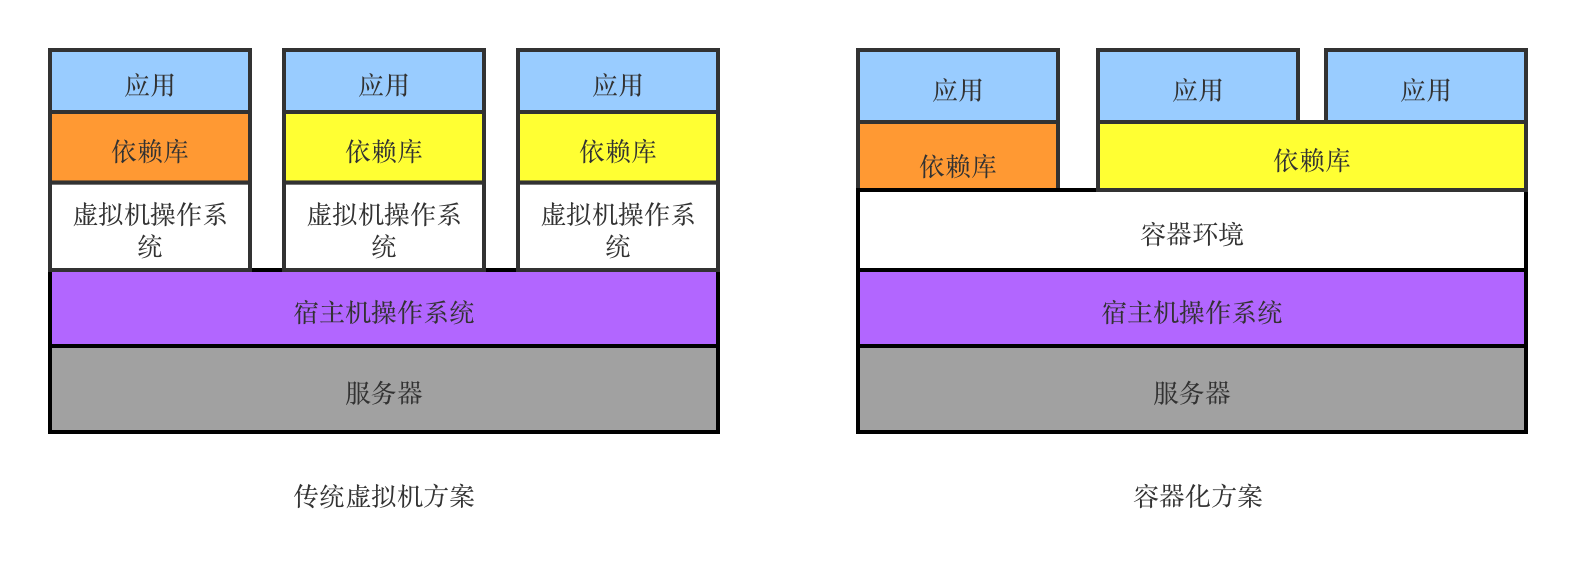
\includegraphics[width=10cm]{images/container.png}
    \caption{容器化vs虚拟机}
    \label{fig:container}
\end{figure}

模型服务化是指将算法和模型等打包成可调用的服务,
目前主流的做法就是利用Docker将模型需要的依赖和环境打包到Docker镜像中,以HTTP或者RPC的方式对外提供调用接口。

\section{本章小结}
在本章中,首先介绍了下一章将要用到的技术探针方法,然后介绍了相关人脸检测算法以及本文用到的特征提取算法、诊断模型等,
最后介绍了本文在系统设计中用到的容器化技术和相关系统设计方法。